\documentclass[journal,10pt,twocolumn]{article}
\usepackage{graphicx}
\graphicspath{{./Figures/}}
\usepackage[margin=0.5in]{geometry}
\usepackage[cmex10]{amsmath}
\usepackage{amssymb}
\usepackage{array}
\usepackage{booktabs}
\title{Circle Assignment}
\def\myauthor{G Kumar}
\def\contact{kumargandhamaneni20016@gmail.com}
\def\mymodule{Future Wireless Communication (FWC)}
\date{}
\providecommand{\norm}[1]{\left\lVert#1\right\rVert}
\let\vec\mathbf
\newcommand{\myvec}[1]{\ensuremath{\begin{pmatrix}#1\end{pmatrix}}}
\newcommand{\mydet}[1]{\ensuremath{\begin{vmatrix}#1\end{vmatrix}}}
\providecommand{\brak}[1]{\ensuremath{\left(#1\right)}}
\usepackage{graphicx}
\graphicspath{{./images/}}
\usepackage[colorlinks,linkcolor={black},citecolor={blue!80!black},urlcolor={blue!80!black}]{hyperref}
\usepackage[parfill]{parskip}
\usepackage{lmodern}
\usepackage{tikz}
\usepackage{physics}
\usepackage{tabularx}
\usetikzlibrary{calc}
\usepackage{amsmath}
\usepackage{amssymb}
\renewcommand*\familydefault{\sfdefault}
\usepackage{watermark}
\usepackage{lipsum}
\usepackage{xcolor}
\usepackage{listings}
\usepackage{float}
\usepackage{titlesec}
\providecommand{\mtx}[1]{\mathbf{#1}}
\titlespacing{\subsection}{1pt}{\parskip}{3pt}
\titlespacing{\subsubsection}{0pt}{\parskip}{-\parskip}
\titlespacing{\paragraph}{0pt}{\parskip}{\parskip}
\newcommand{\figuremacro}[5]{
    \begin{figure}[#1]
        \centering
        \includegraphics[width=#5\columnwidth]{#2}
        \caption[#3]{\textbf{#3}#4}
        \label{fig:#2}
    \end{figure}
}
\lstset{
frame=single, 
breaklines=true,
columns=fullflexible
}
\thiswatermark{\centering \put(0,-105.0){
\includegraphics[scale=0.35]{iith}} }
\author{\myauthor\hspace{1em}\\\contact\\IITH\hspace{0.5em}-\hspace{0.5em}\mymodule}
\begin{document}
\maketitle
\section*{Problem}
Let $x^2+y^2-4x-2y-11=0$ be a circle.A pair of tangents from point(4,5) with pair of radii form a quadrilateral of area.........
\section*{Solution}

\begin{figure}[h]
\centering
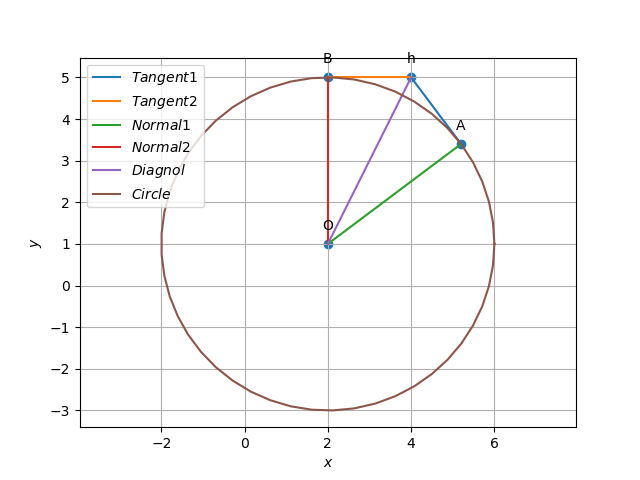
\includegraphics[width=1\columnwidth]{circle.png}
\caption{Circle with center O and points A,B \& h}
\label{fig:Circle}
\end{figure}
\begin{tabular}{|c|c|c|}
  \hline
  \textbf{Symbol}&\textbf{Value}&\textbf{Description}\\
  \hline
  $\vec{h}$&$\begin{pmatrix}
  4\\5
  \end{pmatrix}$&  external point\\
  \hline
  $\vec{O}$&$\begin{pmatrix}
  2\\1
  \end{pmatrix}$&centre of circle\\
  \hline
  $\vec{A}$&$\begin{pmatrix}
  5.201\\3.403
  \end{pmatrix}$& point of contact\\
  \hline
  $\vec{B}$&$\begin{pmatrix}
  2\\5.008
  \end{pmatrix}$& point of contact\\
  \hline
  
\end{tabular}
\subsection*{Step 1}
\large{Given,equation of circle and point are,} 
   \begin{equation}
   x^2+y^2-4x-2y-11=0, h=(4,5)
   \end{equation}
   \large{The equation of a conic section is given by,}
   \begin{align}
   \vec{x}^{\top}\vec{V}\vec{x}+2\vec{u}^{\top}\vec{x}+f=0
   \end{align}
   \large{So,equation of circle in (1) can be written in form of equation(2) and point P in vector form as,}
   \begin{align}
   \vec{x}^{\top}\vec{x}+2\myvec{-2&-1}\vec{x}-11=0, \vec{h}=\myvec{4\\5}
   \end{align}
   From this,
   \begin{align}
   \vec{V}=\myvec{1&0\\0&1}\vec{u}=\myvec{-2\\-1}, \vec{O}=\myvec{2\\1}, f=-11
   \end{align}
   \large{If $\vec{V}^{-1}$ exists, given normal vector $\vec{n}$, the tangent points of contact to equation(2) are given by,}
\begin{align}
\vec{q_i}=\vec{V}^{-1}(k_i\vec{n}-\vec{u})^T \\
where,k_i=\pm \sqrt{\frac{f_0}{\vec{n}^T\vec{V}^{-1}\vec{n}}}\\
f_0=\vec{u}^T\vec{V}^{-1}\vec{u}-f\\
\end{align}  
 The normal vectors of tangents from a point $\vec{h}$ to the conic(2) are given by'
   \begin{align}
   \vec{n_1}=\vec{P}\myvec{\sqrt{\lambda_1}\\ \sqrt{\lambda_2}},\vec{n_2}=\vec{P}\myvec{\sqrt{\lambda_1}\\ -\sqrt{\lambda_2}}
   \end{align}
where $\lambda_i,\vec{P}$ are eigen parameters of 
\begin{align}
\sum=(\vec{V}\vec{h}+\vec{u})(\vec{V}\vec{h}+\vec{u})^T-\vec{V}(\vec{h}^T\vec{V}\vec{h}+2\vec{u}^Th+f)
\end{align}
   So, by solving above equation,
   \begin{align}
   \vec{n_1}=\myvec{1.333\\1},\vec{n_2}=\myvec{0\\1}
   \end{align} 
   By solving equation(6), using (4),(7) and (11), we get,
   \begin{align}
   k=\pm0.8968
   \end{align}
   Solving equation(5), using (4),(11) and (12), we get,
   \begin{align}
   \vec{A}=\myvec{5.201\\3.403}\hspace{0.4em} and\hspace{0.5em}\vec{B}=\myvec{2\\5.008}
   \end{align}
   Now, Area of $\triangle\vec{OBh}$ is given by,
   \begin{align}
   ar(\triangle\vec{OBh})=\frac{1}{2}\norm{\vec{BO}\times\vec{Bh}}
   \end{align}
   \begin{align*}
   ar(\triangle\vec{OBh})=\frac{1}{2}\norm{(\vec{B-O})\times(\vec{B-h})}
   \end{align*}
   \begin{align*}
   ar(\triangle\vec{OBh})=\frac{1}{2}\norm{\myvec{\myvec{2\\5.008}-\myvec{2\\1}}\times\myvec{\myvec{2\\5.008}-\myvec{4\\5}}}
   \end{align*}
   \begin{align}
   \implies\hspace{0.8em}ar(\triangle\vec{OBh})=4 squ
   \end{align}
   Area of Quadrilateral $\vec{OBhA}$ is given by,
   \begin{align}
   ar(\vec{OBhA})=2ar(\triangle\vec{OBh})
   \end{align}
   Therefore,
   \begin{align}
   ar(\vec{OBhA})=8squ
   \end{align}
\end{document}